\documentclass[english,a4paper]{scrartcl}
\usepackage[T1]{fontenc}
\usepackage[latin1]{inputenc}
\usepackage{amsmath,amssymb,graphicx,url,parskip,
capt-of,textcomp}
\usepackage{hyperref,natbib,array,varioref,xspace}

\usepackage[version=3]{mhchem}

%\usepackage[english]{babel}
%\usepackage{lmodern}

% Minion and Myriad fonts
%\usepackage[minionint,mathlf]{MinionPro}
%\renewcommand{\sfdefault}{Myriad-LF}
\usepackage{lmodern}

%\renewcommand{\familydefault}{\sfdefault}
%\fontfamily{verdana}\selectfont 

\usepackage{microtype}

\pagestyle{empty}


\bibpunct{(}{)}{;}{a}{,}{,}
\renewcommand{\labelenumi}{(\roman{enumi})}

\begin{document}

\section*{The Project BIOGAS-EXPERT: Motivation}

For Schleswig-Holstein, as an agricultural site, the utilization of biomass for energy production has already become an indispensable segment of the agricultural production process. 
Since the Renewable Energy Law has come into effect, and particularly its 2009 revision, Schleswig-Holstein, similar to the entire republic, is recording an increasing trend for the installation of biogas plants. In 2005, approximately 46 Biogas plants were operating (Holz, 2006), which accounted for 1.3 percent of the 3500 plants operating throughout Germany. In 2010 more than 200 biogas plants generate energy, which is nearly 5 percent of the plants located in Germany. It can be assumed that, further more plants in Schleswig Holstein will be approved.
A long-term sustainable economic development of biogas production in Schleswig-Holstein requires an appropriate provision of suitable substrates. In terms of a circulatory system, this involves recycling of the fermented substrate (residues from the fermentation process). However, the Federal Environment Agency judges the extensive cultivation rather critically, because

\begin{enumerate}
\item high biomass yields require an equally high input of fertilizer and pesticides, which in Schleswig-Holstein have been under fire with regard to the standards established by the European Water Framework Directive, and 
\item with respect to the residue application, the allocation of biomass plants leads to regional "hot spots", which, already today, are discernible in the region of Schleswig, and 
\item due to fuel - food competition for arable land.  
\end{enumerate}

As a consequence, the production of plant material destined for the fermentation takes place to some extent far off the biogas plants while the fermentation residues are applied close to the fermenter. This is to be considered critically with respect to energy yield, as well as to the resulting nitrogen allocations in certain regions. Due to a high nitrogen application level beyond the prescribed time limits of fermentation residues to agricultural land (fertilization ordinance), critics give rise to the fear that the leachate, in particular, will be polluted with nitrogen. Such a scenario would thwart the guidelines of the European Water Framework Directive and force the legislator to take medium-acting measures to guarantee the implementation of the European Water Framework Directive by 2015.
Well founded scientific data of polluted leachate concerning the application of fermentation residues are not presented in Germany so far. Furthermore, the storage and application of fermented substrate will bring about unwanted greenhouse gas emissions such as ammonia, nitrous oxide, and methane. A sustainable optimisation of biomass production must consider environmental effects, particularly with regard to climate and groundwater protection in the process chain.

Biogas plant operators need expert knowledge guaranteeing high quality and security of the control of bio energy plants, as well as the ability to precisely document each phase in the process chain. Both qualities are imperative for the success at a macroeconomic level and sustainable operation. 


\section*{Overview of the joint research project}

Because the aim of this project is to determine the complete N-nutrient cycle of the economic system "biogas plant", different subprojects have been established which are dealing with the following thematic topic:

\begin{labeling}{Subproject 1:}
\item[Subproject 1:] Characterization of substrate quality and methane yield in a modular process
laboratory.
\item[Subproject 2:] Optimization of the yield potential and nutrient utilization efficiency in biomass production systems destined for biogas plants operating under the climatic conditions of Schleswig-Holstein.
\item[Subproject 3:] NH3-losses after application of fermentation residues of biogas plants in differing crop rotation systems in Schleswig-Holstein.
\item[Subproject 4:] Effects of fermentation residues on the emission of climate-relevant trace gases (\ce{CH4} and \ce{N2O}).
\item[Subproject 5:] Effects of fermentation residues on the Nitrogen leaching potential of different crop-rotations.
\end{labeling}

Intensive cooperation is essential to each subproject. Each process, as illustrated below, depends on a good cooperation among its staff as well as on the farmers involved in the process, as most of the field work can only be managed as a team.

The following illustration describes schematically the individual projects. 
\minisec{}
\begin{center}
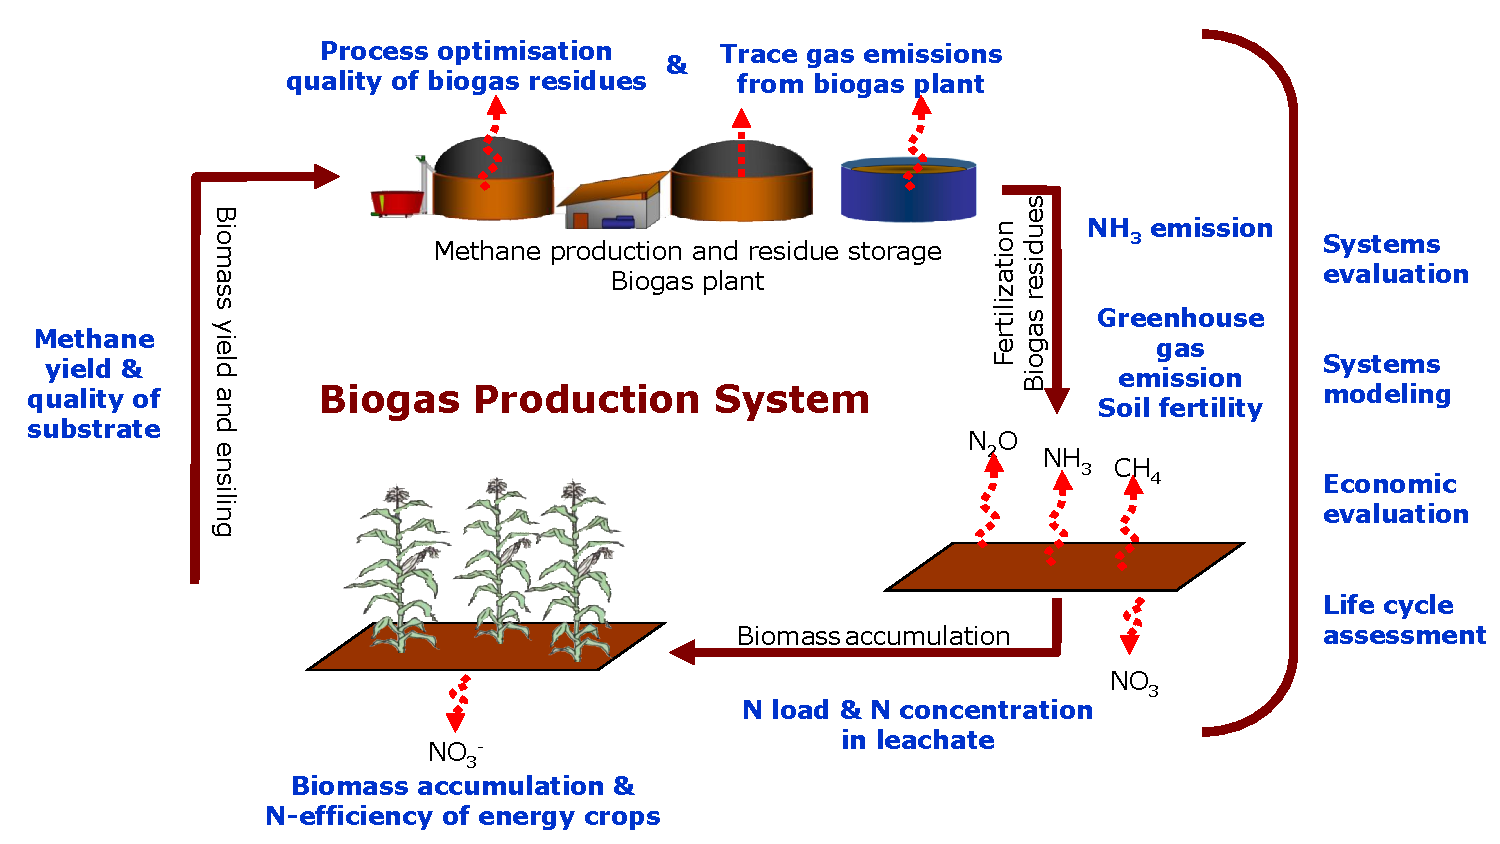
\includegraphics[width=\textwidth]{biogas}  
\end{center}


\section*{Subproject 2}
\subsection*{Optimization of the yield potential and nutrient utilization efficiency in biomass production systems destined for biogas plants operating under the climatic conditions of Schleswig-Holstein.}

This subproject is aimed at determining different cultivation systems of bioenergy plants with regard to their performance and their potentials for utilization of fermentation residuals.
For the supply of biomass, the monocropping of maize gains in importance due to its high biomass potential. At least for Schleswig-Holstein, in light of the prevalent favourite precipitation situation  (mean annual precipitation of 700-850mm/a), the following working hypothesis can be formulated: Depending on the soil quality and precipitation situation crop rotations with winter catch crops and whole crop silage  will reach an even higher level of potential methane production, gained from dry matter, than maize in monoculture. 

As a result of this hypothesis, and because the water availability as a function of the location and weather conditions probably constitutes the limiting factor for an extension and intensification of energy crop cultivation systems by means of winter catch-crops and whole crop silage, a further field of interest has evolved, namely the investigation into the performance of energy crop rotations with respect to their water utilization efficiency.
Furthermore, it is assumed that with respect to the availability of nitrogen, the nitrogen use efficiency of processed fermentation residues in crop rotations with winter catch crops exceeds that of maize in monocultures.

Drawing on the data provided from the two Experimental Farms Hohenschulen (Eastern Upland) and Karkendamm (Geest), this project forms the experimental basis for the sub-projects SP3 (\ce{NH3}-Emission), SP4 (\ce{CH4}-, \ce{N2O}-Emission) and SP5 (\ce{NO3}-Loss). 

\minisec{Description}

In two field trials established at the experimental sites maize in monoculture, energy crop rotations (wheat: silage, grain; ryegrass or mustard as winter catch crop; maize) and grassland swards (four cuts) with different fertilizer level have been investigated.

Throughout the vegetation period, studies have been conducted investigating the biomass production, nitrogen assimilation and NUE. Both, destructive and none-destructive samplings have been taken (e.g. LAI 2000 and SPAD).
On the basis of the provided data, modules of dynamic simulation models for the calculation of dry matter production, nitrogen assimilation, and DM-content of the crop species cultivated  are to be adapted to the special conditions of the production of energy crops and, in this sense, improved. Simulations are being carried out by means of the class oriented modelling environment HUME and the modules designed for the calculation of the soil water content and the biomass production (FOPROQ implemented in the HUME model).

%\begin{minipage}[b]{.48\linewidth}
%  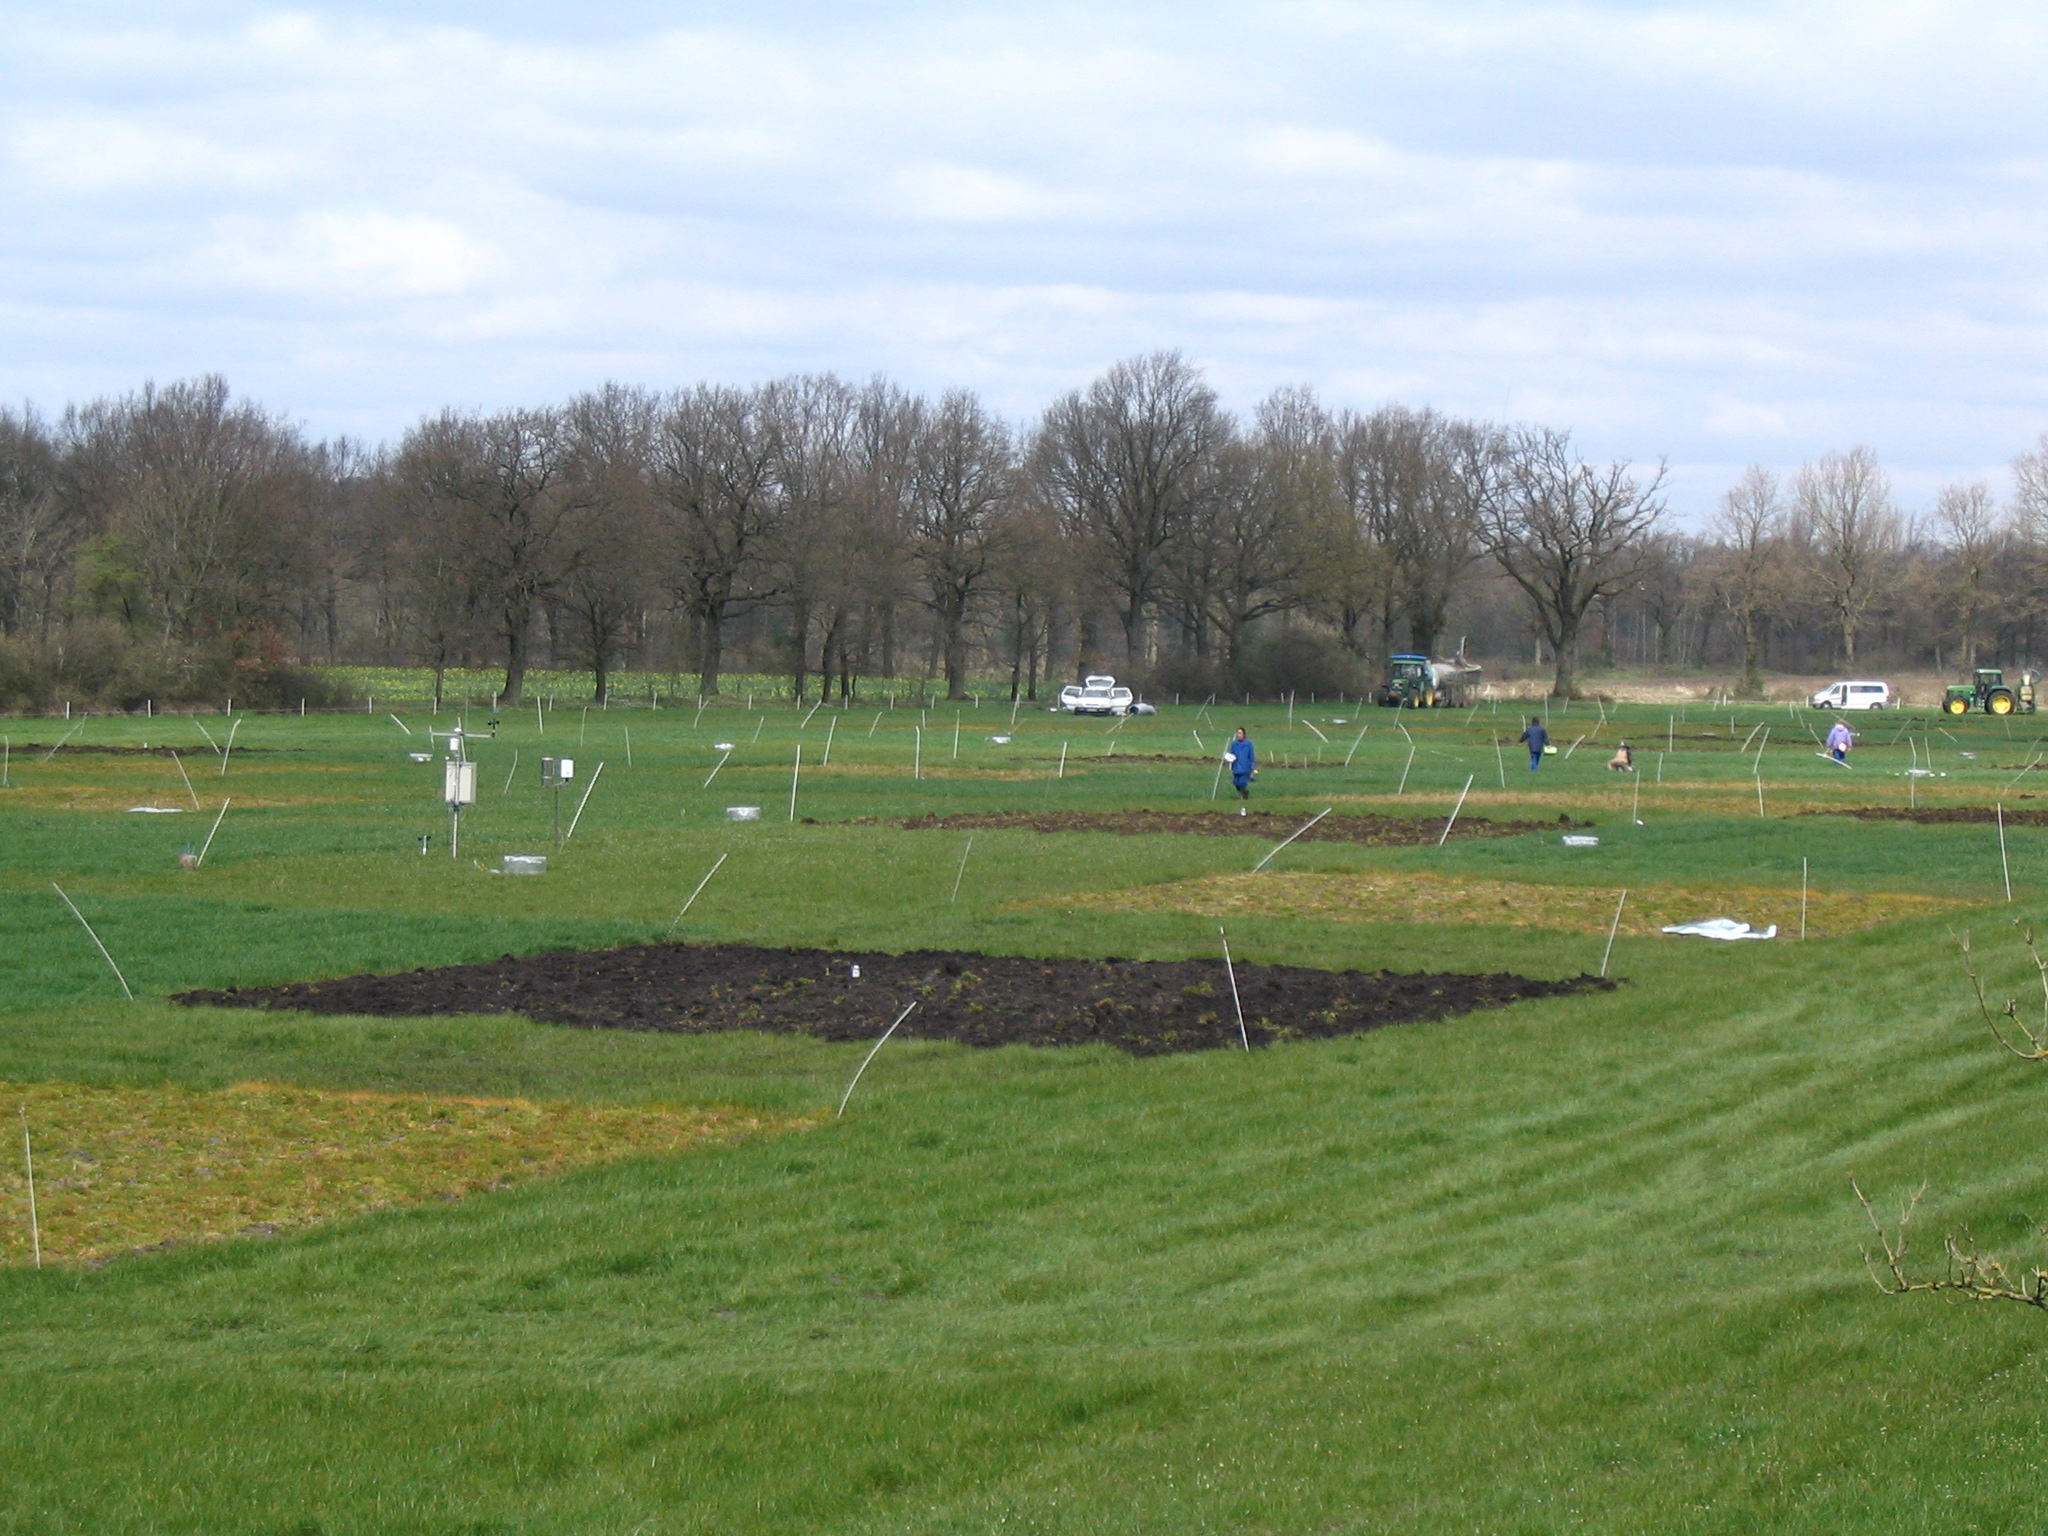
\includegraphics[width=\textwidth]{karkendamm}
%  %\captionof{fugure}{Karkendamm}  
%  Karkendamm
% \end{minipage}
%\hspace{.04\linewidth}% Abstand zwischen Bilder
%\begin{minipage}[b]{.48\linewidth}
%  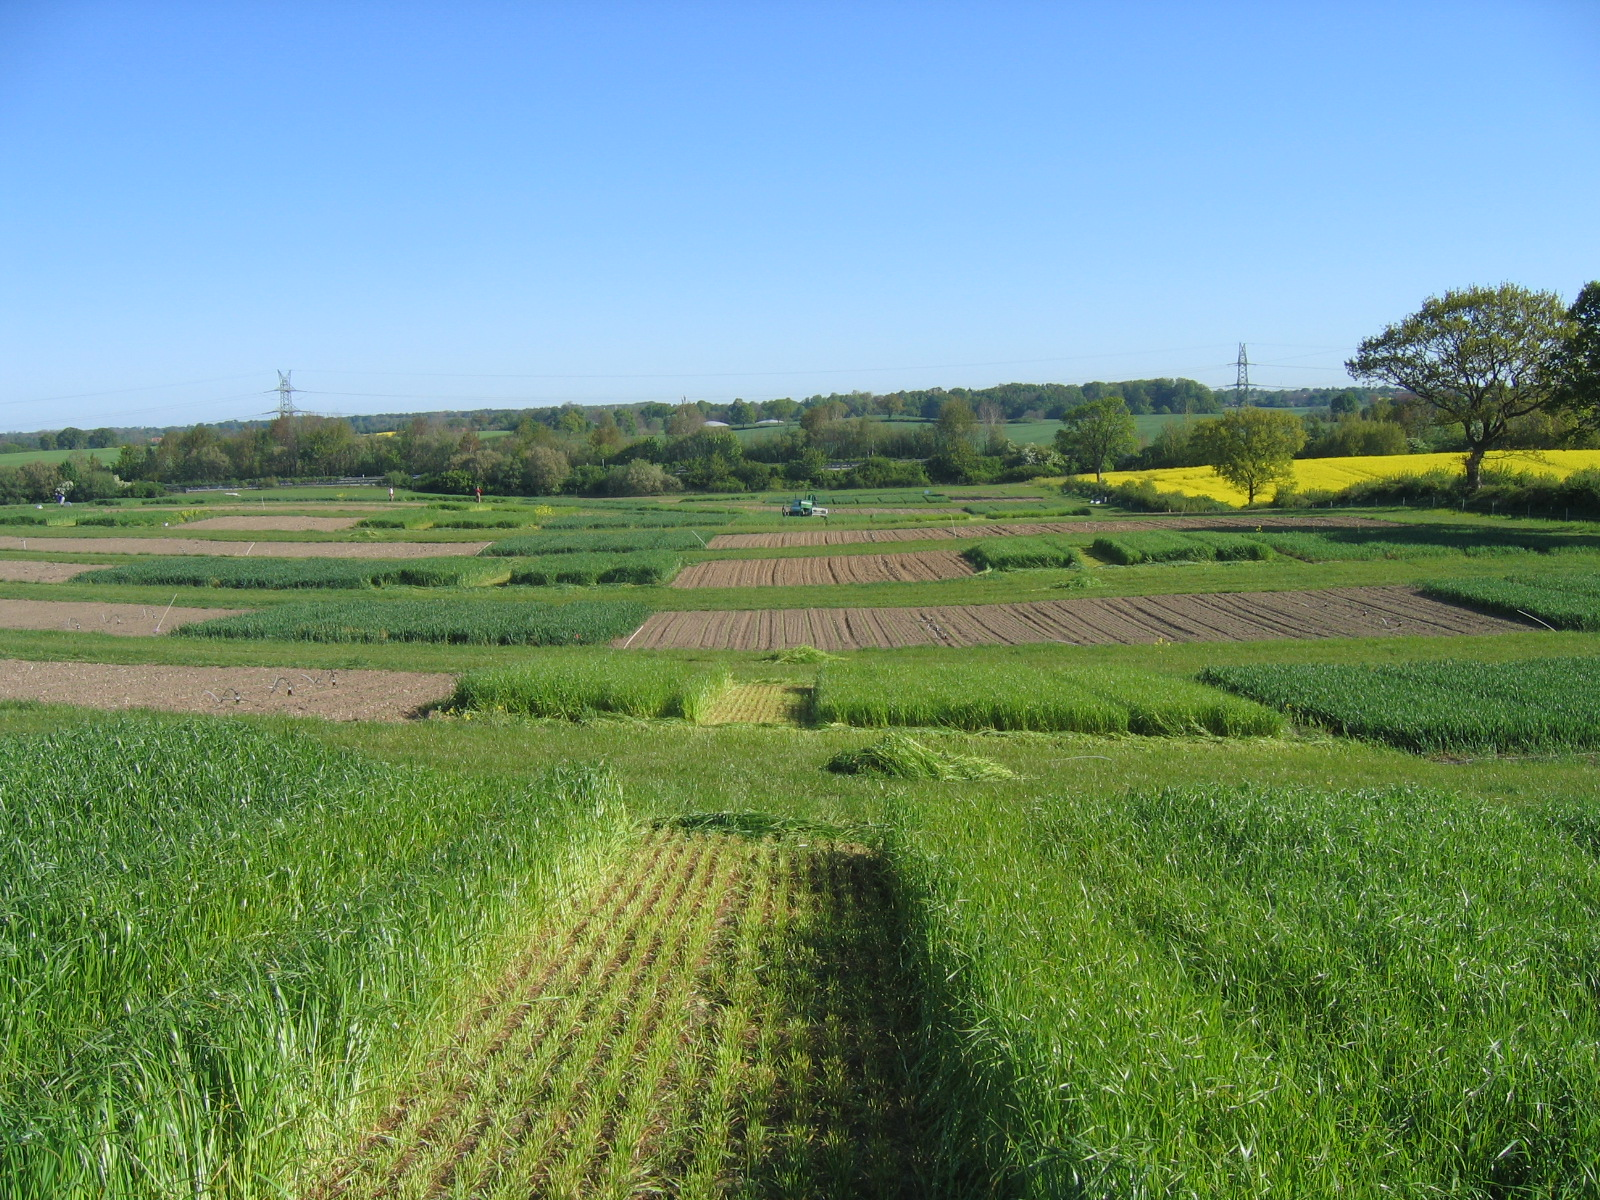
\includegraphics[width=\textwidth]{hohenschulen}   
%  %\captionof{figure}{Hohenschulen}
%  Hohenschulen
%\end{minipage}


\section*{Subproject 3}

\subsection*{\ce{NH3} losses after application of fermentation residues in different crop rotation systems in Schleswig-Holstein.}

\ce{NH3} losses after application of fermentation residues resulting from biogas production, exclusively based on the fermentation process of plant substrates, have hardly been investigated thus far. The object of subproject 3 is the quantification of the \ce{NH3} emission after application of fermentation residuals compared to slurry. It has been assumed that mono fermented slurry exhibit higher pH-values, which promote evaporation of ammonia.

In order to measure the \ce{NH3} emission, three kinds of measuring techniques (see illustrations) are to be established in the course of two field trials at two different locations which are typical for the region of Schleswig-Holstein (Karkendamm and Hohenschulen).  By means of accompanying process studies (pH measurement, measurement of water content, etc.), the mechanism underlying the \ce{NH3} emission will be investigated more closely.

First results have shown that co-fermented slurry exhibit the highest losses of ammonia. A reason for that could be the increased viscosity in comparison to other types of slurry.

\minisec{}

\begin{minipage}[t]{.3\linewidth}
\begin{center}
  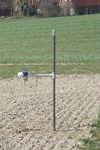
\includegraphics[width=\textwidth]{Clipboard01N}
  \end{center}
 \begin{flushleft}
 {Measurement method 1: "Space-Shuttles" are installed at a defined altitude. The Shuttles contain oxalic acids, which absorb the ammonia from the air.}
 \end{flushleft}
\end{minipage}
\hspace{.05\linewidth}
\begin{minipage}[t]{.3\linewidth}
\begin{center}
  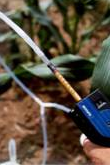
\includegraphics[width=\textwidth]{Clipboard02N}  
  \end{center}
  \begin{flushleft}
  {Measurement method 2: The Dr�ger company, in L�beck, produces tubes which measure the ammonia content in the air.} % 
  \end{flushleft}
\end{minipage}
\hspace{.05\linewidth}
\begin{minipage}[t]{.3\linewidth}
\begin{center}
  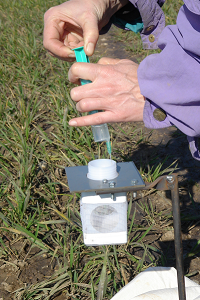
\includegraphics[width=\textwidth]{Clipboard03N}
  \end{center}
  \begin{flushleft}
  {Measurement method 3: Small samplers are placed on the   experimental plots. They are filled with sulphuric acid which, similar to the oxalic acids, absorbs the ammonia gas from the air.}%
  \end{flushleft}
\end{minipage}


\section*{Subproject 4}
\subsection*{Effects of fermentation residue application on the emission of climatic relevant trace gases (\ce{CH4} and \ce{N2O}) and carbon-/humus balance of the soil}

The planned investigations are divided into two thematic fields dealing with the sustainability of the application of biogas slurry in agriculture. In addition, both thematic fields can draw on extensive experiences with conventional slurry.

First, through field- and pot experiments, the effects of biogas slurry on the emission of greenhouse gasses (\ce{CH4} and \ce{N2O}) are to be examined. These tests will be embedded in the major plant cultivation experiments of the overall project. The object is to record the emissions over the period of one year, immediately following the application of the biogas slurry. Furthermore, important interactions with different kinds of mineral fertilisers will be investigated. 

The second field deals with the determination of the effects of biogas slurry on the humus content of the soil (soil organic matter), which is an important parameter of the soil fertility. At this point the working hypothesis is that biogas slurry exhibits a lower carbon content and a tighter C/N relation (depending on the substrates/co-ferments) compared to conventional slurry. 
Because of the specific characteristics of biogas slurry (increased $NH_4$ ratio, lower C ratio) a different turnover rate for nitrous oxide emissions as well as for the preservation of the humus (carbon content) is to be expected.
\minisec{}
\begin{center}
\includegraphics[width=\textwidth]{ring} 
\end{center}

\section*{Subproject 5}

\subsection*{Effects of biogas residue application on the N-loss of different crop rotations and soil types}

%\begin{minipage}[b]{.74\linewidth}
The object of this study is the analysis and determination of the potential of nitrate leaching after the application of biogas slurry (co-fermentation, mono-fermentation). Here the focus is on determining the N-leachate and comparing it to the "performance" of conventional fertilizers (cow and pig manure). Important goals include the development of optimisation strategies for the energy plant cultivation and its evaluation with respect to groundwater protection on a regional scale.

So far, the effects of a long retention time of animal fertilizer in the fermenter have not been sufficiently examined.
Data acquisition draws from three leachate periods. Within these periods, field experimental plots are being sampled and leachate is being taken at a depth of 60 cm. In addition, samples of all types of slurry thus applied are collected and examined with reference to the parameters related to this project (N, P, K, pH, TS, Visc.). Prior to each application of slurry, the "slurry producer" takes a sample, which he examines with respect to its N content, in order to calculate the quantity he must actually apply. Results concerning to this Project are presented on this convention.

\par
\textbf{Poster: 2.1.42} \par
\textbf{Nitrogen leaching after application of biogas residue}

\minisec{}
%\end{minipage}
%\hspace{.02\linewidth}% Abstand zwischen Bilder
\begin{minipage}[t]{.74\linewidth}
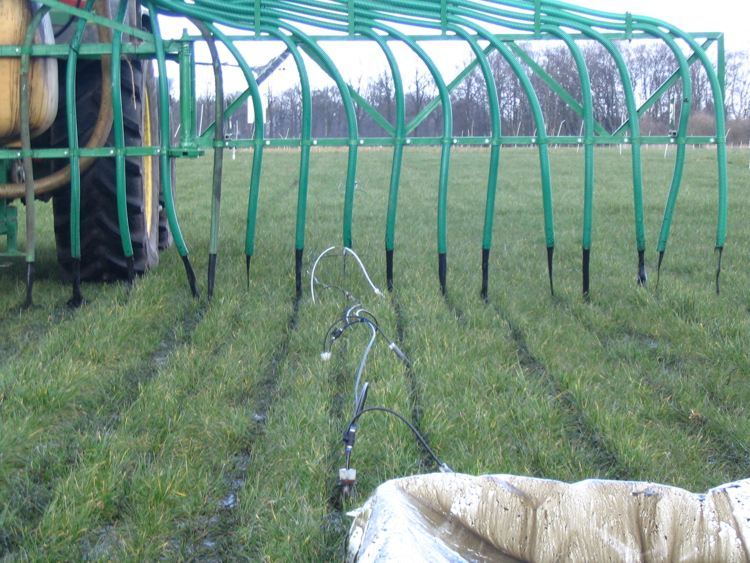
\includegraphics[height=225pt]{duengung} 
\end{minipage}
\hspace{.02\linewidth}% Abstand zwischen Bilder
\begin{minipage}[t]{.24\linewidth}
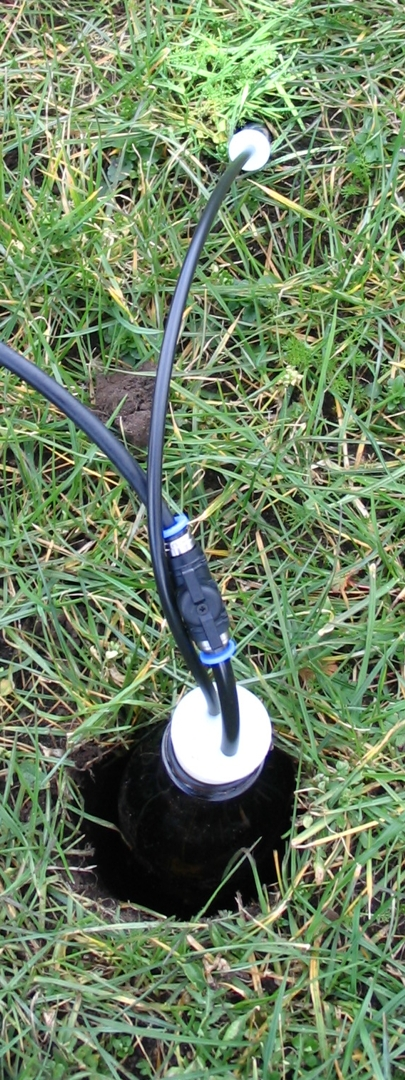
\includegraphics[height=225pt]{ding}  
\end{minipage}




 


%\bibliographystyle{plainnat}
%\bibliography{niko}

\end{document}
